\chapter{Resultater og diskusjon}

Her følger noen eksempler på tabeller og figurer. Alle er hentet fra \cite{paraschiv_bankruptcy_2021}.

\begin{table}[h]
  \centering
\captionof{table}{\textbf{Simulation of a competitive credit market with two banks -- general versus industry-specific datasets}}\label{tab:simulation_1:industry}
    \begin{tabular}{l|rr}
    \hline\hline
          & \textbf{LAS} & \textbf{LIN}  \\
          \hline
    \textbf{Market share of each bank in EUR (\%)} &  50.8  &  49.1   \\
    \textbf{Share of bankrupting borrowers in portfolio (\%)} &  2.7  & 1.9  \\
    \textbf{Share of bankrupting borrowers in the market (\%)} & 57.1  &    34.6  \\
    \textbf{Revenue} &    55,854.8  &    50,954.0 \\
    \textbf{Loss} &    24,169.3  &    17,302.1   \\
    \textbf{Profit} &    31,685.5  &    33,652.0   \\
    \textbf{Profit margin (\%)} & 56.7  & 66     \\
    \textbf{Return on assets (ROA) (\%)} & 0.3   & 0.4    \\
    \textbf{Return on risk-weighted assets (RORWA) (\%)} & 0.5   & 0.6   \\
    \hline\hline
    \end{tabular}
    % \bigskip
  \caption*{Tabelltekst her. Teksten bør være så utfyllende at leseren skjønner hva tabellen forteller uten å måtte se i hovedteksten.}
\end{table}



\begin{figure}[h]
\captionof{figure}{\textbf{Stability of variable selection}}\label{fig:number of unique input variables}
	\centering
	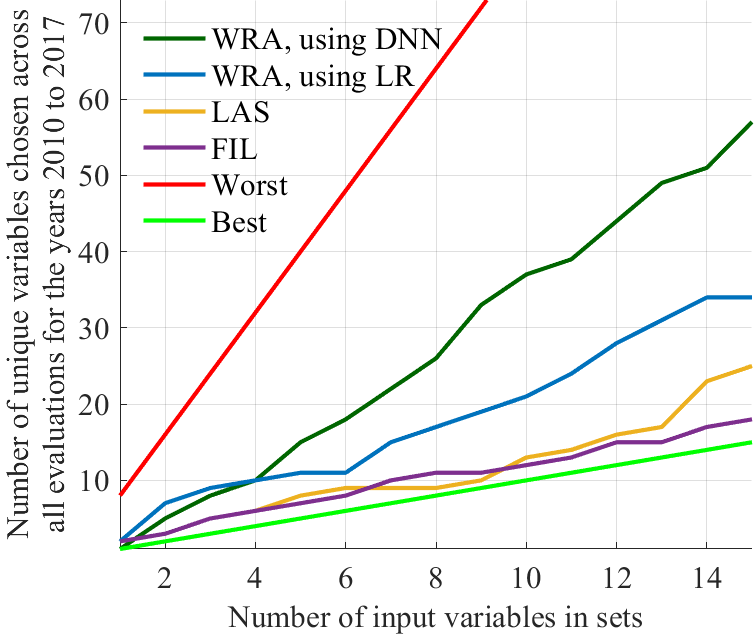
\includegraphics[width=0.49\linewidth]{images/unique_input_variables.png}
	% \bigskip
 	\caption*{Figurtekst her. Teksten bør være så utfyllende at leseren skjønner hva figuren forteller uten å måtte se i hovedteksten.}
\end{figure}


\begin{figure}[h]
  	\begin{center}
  	\captionof{figure}{\textbf{Total cumulative amount lent within percentiles of amount borrowers are willing to borrow -- General versus industry-specific variable sets}}
  	\label{fig:simulation_proportions}
  	\captionsetup{justification=centering}
  	 \begin{subfigure}[t]{0.47\linewidth}
  	 \vspace{0.4cm}
  	        \caption*{\large Panel A}
  	        \vspace{-0.3cm}
    		\includegraphics[width=\linewidth]{"images/pst_cum_captured_non_bankrupt".png}
  	\end{subfigure}
 	\begin{subfigure}[t]{0.47\linewidth}
 	\vspace{0.4cm}
            \caption*{\large Panel B}
            \vspace{-0.3cm}
    		\includegraphics[width=\linewidth]{"images/pst_cum_captured_bankrupt".png}
  	\end{subfigure}
  	\vspace{-0.6cm}
  	\end{center}
  \caption*{Tabelltekst her. Teksten bør være så utfyllende at leseren skjønner hva tabellen forteller uten å måtte se i hovedteksten.}
\end{figure}